\documentclass[DM,lsstdraft,toc]{lsstdoc}

% lsstdoc documentation: https://lsst-texmf.lsst.io/lsstdoc.html

% Package imports go here.
\usepackage{longtable}
\usepackage{makecell}
\usepackage{textcomp}
\usepackage[table]{xcolor}

% Local commands go here.

\newcommand\skipcoloring[0]{%
\global\advance\rownum-1\relax
}

\renewcommand\cellalign{tl}

% Environment for displaying the schema tables in
% a consistent manner. Two arguments are the
% caption and short caption that differ for each table.
% The third argument is the label to use for the table
\newenvironment{schema}[3]{%
\setlength\LTleft{0pt}
\setlength\LTright{\fill}
\begin{longtable}{p{1.3in}lp{0.8in}p{3.5in}}

% First header has a caption with a label
\rowcolor{white}
\caption[#1]{#2
% We don't have proper labels right now.
% \label{#3}
}\\

\hline \rowcolor{white}
\textbf{Column Name} & \textbf{Data type} & \textbf{Unit} & \textbf{Description [UCD]}\\ \hline
\endfirsthead

% Subsequent headers have the caption but no label
\rowcolor{white}
\caption[#1]{#2}\\

\hline \rowcolor{white}
\textbf{Column Name} & \textbf{Data type} & \textbf{Unit} & \textbf{Description [UCD]}\\ \hline
\endhead

\hline \rowcolor{white}
\multicolumn{4}{r}{\emph{Continued on next page}} \\
\endfoot

\hline\hline
\endlastfoot
}{%
\hline
\end{longtable}
}

% To add a short-form title:
% \title[Short title]{Title}
\title{LSST Database Baseline Schema}

% Optional subtitle
% \setDocSubtitle{A subtitle}

\author{%
Jacek Becla
}

\setDocRef{LDM-153}

\date{\today}

% Optional: name of the document's curator
% \setDocCurator{The Curator of this Document}

%\setDocAbstract

% Change history defined here.
% Order: oldest first.
% Fields: VERSION, DATE, DESCRIPTION, OWNER NAME.
% See LPM-51 for version number policy.
\setDocChangeRecord{%
  \addtohist{1}{2007-01-12}{Initial Version.}{Jacek Becla}
  \addtohist{2}{2007-02-14}{General edits.}{Jacek Becla}
  \addtohist{3}{2007-02-21}{General edits.}{Jacek Becla}
  \addtohist{4}{2007-02-27}{General edits.}{Jacek Becla}
  \addtohist{5}{2007-03-05}{General edits.}{Jacek Becla}
  \addtohist{6}{2007-03-07}{General edits.}{Jacek Becla}
  \addtohist{7}{2007-04-09}{General edits.}{Jacek Becla}
  \addtohist{8}{2007-09-05}{General edits.}{Jacek Becla}
  \addtohist{9}{2011-07-04}{General edits.}{Jacek Becla}
  \addtohist{10}{2011-07-14}{General edits.}{Jacek Becla}
  \addtohist{11}{2013-08-02}{Major refresh of the schema to reflect science requirements described in Data Products doc. Added sections about schema evolution, provenance}{Jacek Becla, Kian-Tat Lim}
  \addtohist{12}{2013-09-30}{Resynchronized with the latest Data Products Definition Document (v Sep 23 2013) and corresponding schema.}{Jacek Becla}
  \addtohist{13}{2013-10-10}{TCT approved}{R. Allsman}
  \addtohist{14}{2013-10-18}{Fixed Table of Contents}{Jacek Becla}
}

\begin{document}

% Create the title page.
% Table of contents is added automatically with the "toc" class option.
\maketitle

\section{Schema Format and Documentation}

The LSST Database schema master files are stored in yaml files which are designed to be read by the ``Felis''\footnote{https://github.com/lsst-dm/felis/} schema manipulation tool. The files live in the \texttt{cat} package and are version-controlled via git together with the rest of the LSST software.

The yaml files are designed to contain both the required attributes necessary for instantiating a database table and extra per-column metadata for enabling a richer description of the data, such as additional descriptive text, physical units, or IVOA UCDs. The choice of a yaml format also enables additional metadata attributes to be added as the need arises during development.

The schema tables presented in this document are automatically generated from the yaml files in the \texttt{cat} package.

\section{Stored Procedures and Functions}

We maintain a small set of stored procedures and functions, as well as a set of user-defined functions (UDFs). Since stored procedures and functions typically are vendor-specific, we have tried to limit them to the bare minimum; nevertheless, we now have $\sim10$ such procedures, most related to converting different time formats. The most frequently used functions are written as native user-defined functions for performance and portability reasons. They include support for spherical geometry, photometry conversions, and statistical functions (e.g., median). These spatial functions rely on custom HTM indices to allow fast spatial selections, such as point in circle, polygon or ellipse searches. We are collaborating with the team from Johns Hopkins University that implemented HTM indexing and UDFs for SDSS, and we already incorporated many of their lessons learned into our UDFs (their UDFs were written in C\# for SQL Server, since then the SDSS team converted them to C++ using automated conversion tools.)

Since these UDFs are not LSST-specific and may be of broader interest (to MySQL community and beyond), we maintain them as an open-source project independent from LSST. This project, SciSQL, is hosted on launchpad.net (see \url{https://github.com/smonkewitz/scisql}).

\section{Selected Catalogs}

The baseline schema is driven primarily by the Data Products Definitions Document (LSE-163). The schema can be divided into several logical groups:

\begin{itemize}
  \item Core Catalogs
  \item Metadata Catalogs
  \item Provenance Catalogs
  \item SDQA
\end{itemize}

Here, a catalog refers to a group of closely-related tables that act as a unified dataset from an end user's point of view.

\subsection{Core Catalogs}

The core catalogs can be divided into:
\begin{itemize}
  \item Level 1 Catalogs: DiaObject, SSObject. DiaSource and DiaForcedSource.
  \item Level 2 Catalogs: Object, Source, ForcedSource.
\end{itemize}

\textbf{DiaObject} table contains information about astronomical objects measured on difference images. For reproducibility reasons (described in LDM-135, chapter 3.1), we expect to create a new row each time there is an update to a diaObject, thus the total number of rows in that table is higher than the unique number of diaObjects. 

\textbf{SSObject} table contains information about Solar System (also called moving) objects.

\textbf{DiaSource} table contains information about individual measurements of astronomical objects on different images.

\textbf{DiaForcedSource} contains photometry measurements about low signal-to-noise detections done on individual difference image exposures in each place where an object was detected on a previous difference image within one month.

\textbf{Object} Catalog contains information about static astronomical objects measured on a stacked image. It is the most commonly used catalog.

\textbf{Source} Catalog contains information about high signal-to-noise (>5 sigma) detections on single frame images.

\textbf{ForcedSource} table contains photometry measurements about low signal-to-noise detections done on individual exposures in each place where an object was detected on a stacked image. Due to the nature of these detections only a few parameters can be measured, thus the table is very narrow, however it is by far the largest in terms of row-count.

\textbf{DiaObject\_To\_Object\_Match} table keeps a mapping of diaObjects to nearby objects, used primarily for user data analysis. For rapid real-time queries we maintain three nearbyObj columns in DiaObject.

\subsubsection{Sizes}

The table below provides a rough count (size, rows, columns) for core tables (in the last Data Release, counting data only, e.g., size of persistent overheads such as indices is not reflected here). The exact numbers for each DR can be found in LDM-141.

\begin{tabular}{lccc}
  \hline\hline
  Table & Size [TB] & Rows  [billions] & Columns \\
  \hline\hline
  Object (narrow) & $\sim107$ & $\sim47$ & $\sim330$ \\
  Object (all extras) & $\sim1,200$ & Largest $\sim1,500$ & $\sim7,650$ \\
  Source & $\sim5,000$ & $\sim9,000$ & $\sim50$ \\
  ForcedSource & $\sim1,900$ & $\sim50,000$ & 6 \\
  SSObject & $\sim0.003$ & 0.006 & $\sim80$ \\
  DiaObject & $\sim27$ (76 max) & $\sim15$ unique ($\sim44$ max) & $\sim260$ \\
  DiaSource & $\sim23$ & $\sim45$ & $\sim70$ \\
  DiaForcedSource & $\sim13$ & $\sim300$ & 8 \\
  \hline
\end{tabular}

We expect to keep refining the baseline schema extensively through LSST’s construction, and will likely end up adding a small number of additional columns we haven’t thought about so far. Since the schema is used for cost estimation, such changes would increase overall size of the database (and consequently, the cost), so we have reserved in the costing model (LDM-141) 25\% of each table size\footnote{With the exception of ForcedSource and DiaForcedSource} for yet-unknown columns. Further, the costing model assumes a 3\% increase in row size for each Data Release.

\subsubsection{Partitioning}

To optimize disk I/O and ensure frequently accessed columns are collocated, and to avoid unnecessary I/O, selected Catalogs are \textit{vertically partitioned}.

The Object Catalog is partitioned vertically into the following tables: 

\begin{itemize}
  \item Object --- a table with $\sim$330 most frequently used columns. This table is expected to contain $\sim$47 billion rows by the end of the survey, containing $\sim$48\% in the first data release.
  \item Object\_APMean --- a very narrow table containing aperture photometry mean values, on average $\sim$8 per object.
  \item Object\_Periodic --- a very narrow table containing definitions of periodic features, on average $\sim$32 per object.
  \item Object\_NonPeriodic --- a very narrow table containing definitions of non-periodic features, on average $\sim$20 per object.
  \item Object\_Extra --- a very wide table with remaining, less frequently used columns, such as covariances for 2 models (Point Source and Bulge+Disk), and Bulge+Disk samples. These are packed into 3 blobs, 66, 168, and 7,200 elements in each blob respectively. Packing is driven by expected access pattern: entire set of elements in a blob or nothing will be accessed. There will be one such row for each row in the Object table.
\end{itemize}

The Source Catalog consists of two tables: Source and Source\_APMean, the latter is similar to Object\_APMean.

Since managing trillions of rows in a single table is close to impossible, in addition to vertical partitioning, all core catalogs will be horizontally partitioned, The Level 1 catalogs will be partitioned by time into a small set of tables, and all large Level 2 catalogs will be partitioned spatially into $\sim$20,000 partitions for each table. Further details related to horizontal partitioning of these tables are discussed in LDM-135 (\textit{LSST Database Design}).

\subsubsection{Diagram}

The diagram below depicts all core tables, and their relations.

\begin{figure}
  \centering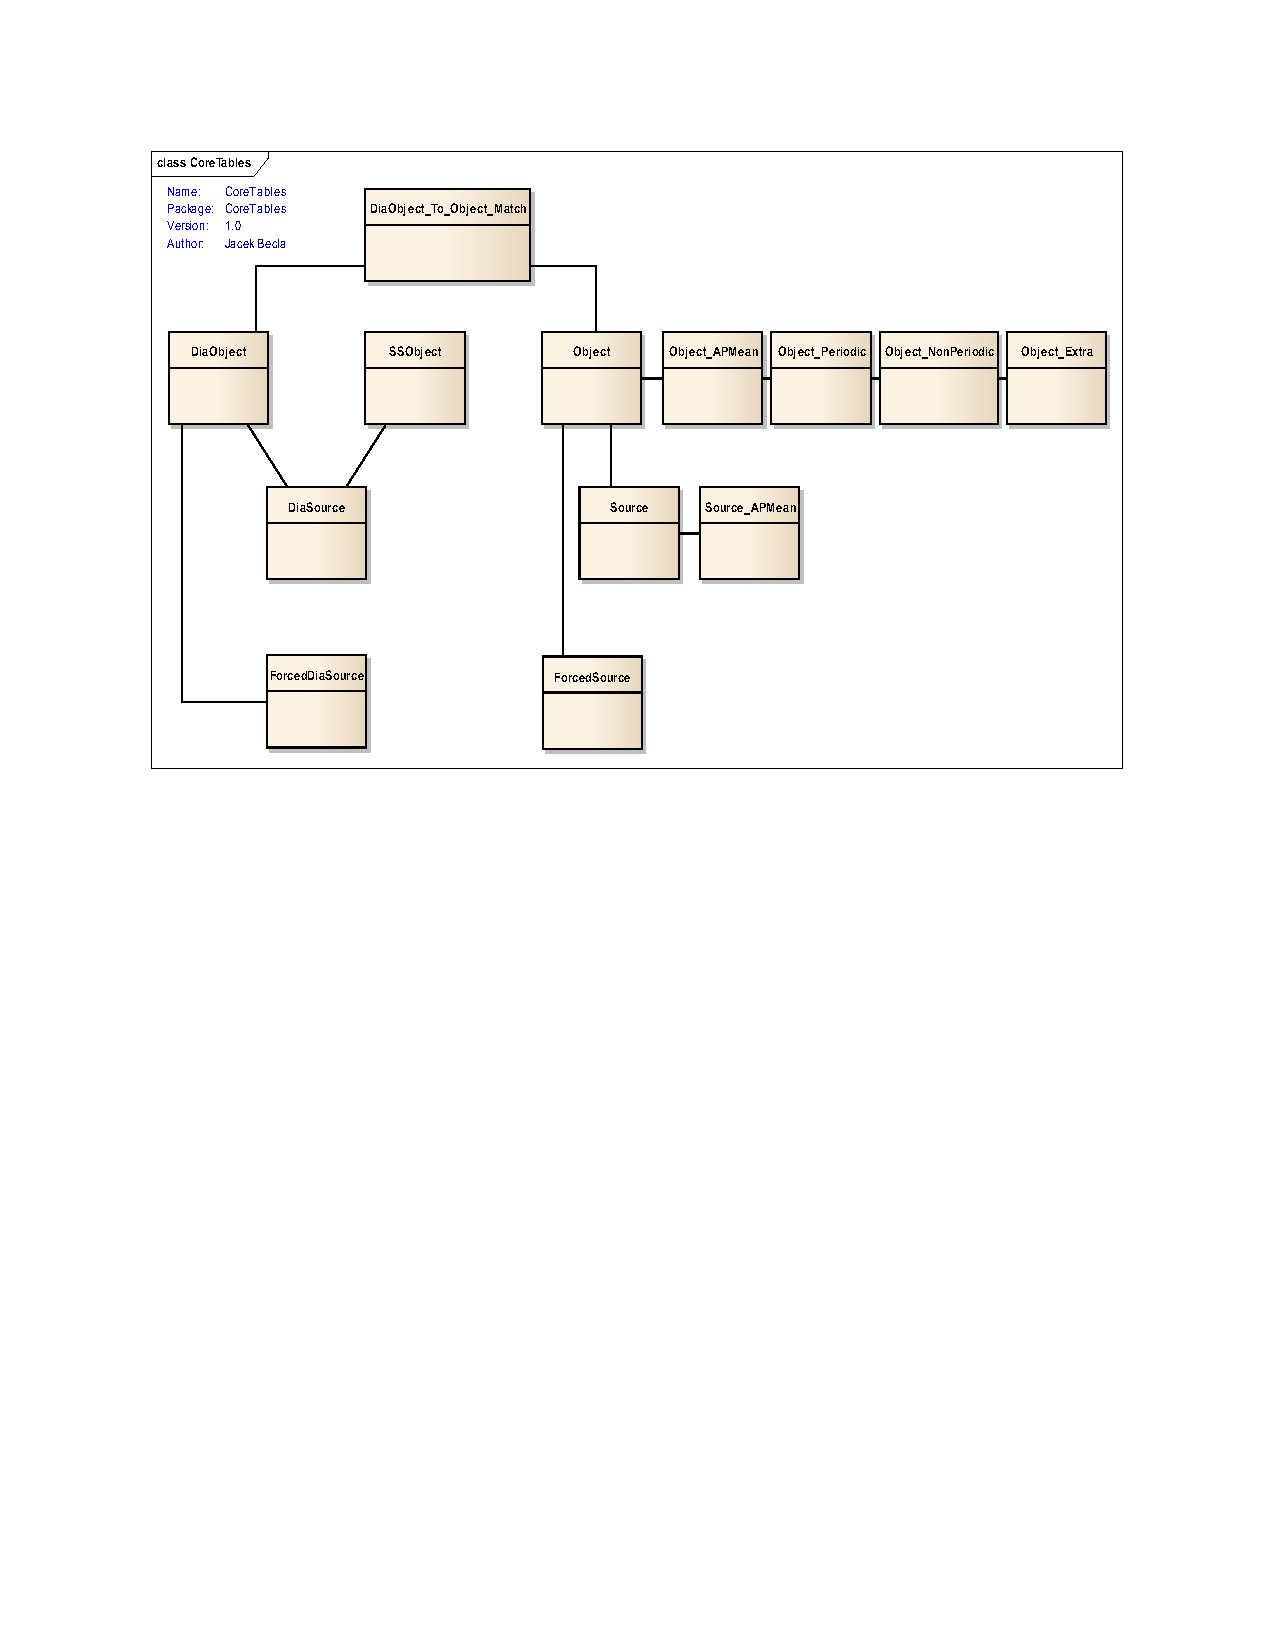
\includegraphics[scale=0.80]{diagrams/coretables}
  \caption{Core table relationships}
\end{figure}

\subsection{Metadata Catalogs}

Metadata catalogs contains information about LSST ``raw exposures'' and ``science calibrated visits''. Information is tracked at different levels:

\begin{itemize}
  \item focal plane (entire exposure/visit),
  \item raft (raft = 9 ccds)
  \item ccd (there are 189 ccds per focal plane)
  \item amp (there are 16 amplifiers per ccd).
\end{itemize}

When appropriate, we denormalize information into ``lower-level'' table (eg, information from ccd-level is repeated for each amp) to avoid extraneous joins for common accesses.

In addition to fully structured tables, for selected tables we expect to maintain an additional table with key-value pairs. This will allow us to introduce additional ``columns'' without altering corresponding table's schema (at the cost of degraded performance). This might be particularly handy when trying to determine what information would be particularly useful to derive from the existing columns. Periodically, most commonly used key-value pairs will be converted into regular columns.

In addition, we maintain a table that maps raw exposures to visits. Typically it will contain two rows for each visit.

\subsubsection{Sizes}

Size of the metadata tables is not posing any major challenge. LSST is expected to produce $\sim$one thousand visits per night, which leads to $\sim$3 million visits during 10 year lifetime of the survey.

\subsubsection{Diagram}

The diagram below depicts the metadata tables, and their relations.

\begin{figure}
  \centering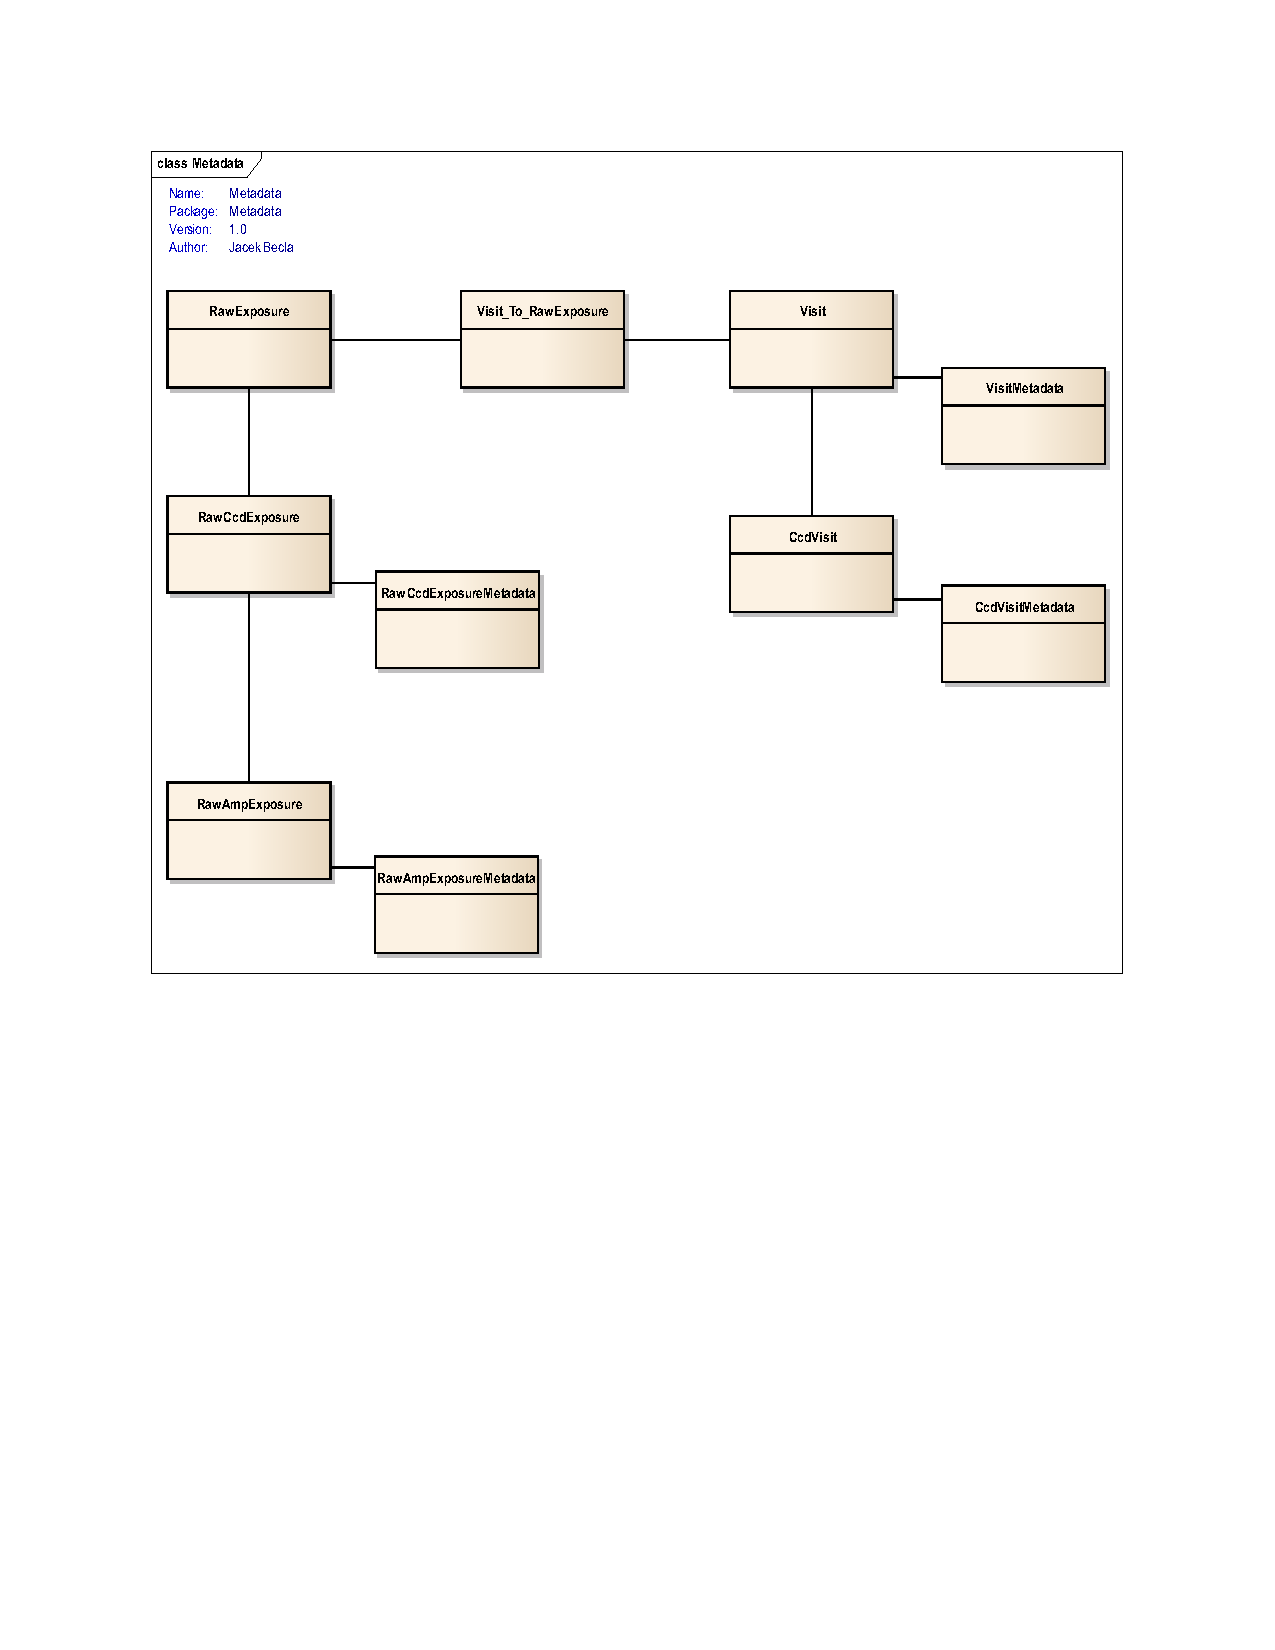
\includegraphics[scale=0.8]{diagrams/metadata}
  \caption{Metadata table relationships}
\end{figure}

\subsection{Provenance}

In LSST, we define Provenance as execution trace, or in other words information ``how we came up with the data''. Provenance will be used primarily:
%
\begin{itemize}
  \item to help with data QA, for example to detect which parts of data were affected by a faulty algorithm or a bad node,
  \item as a recipe how to regenerate intermediate results.
\end{itemize}

Specifically, Provenance is responsible for capturing configuration of:
%
\begin{itemize}
  \item software (which pipelines were run on given data, what processing stages were part of each pipeline, what versions of algorithms were used, how was processing parallelized and on which computing node each piece was executed etc) and
  \item hardware (what was the configuration of focal plane, each raft, ccd, amplifier, filter etc).
\end{itemize}

\subsubsection{Size}

In terms of size, we expect provenance to be a very small fraction of the entire data set. The largest contribution is an 8-byte column we are adding for every core tables (with the exception of DiaForcedSource table, as it will have the same provenance as its corresponding DiaSource table), and selected metadata tables. Note that in some cases, in particular for the very narrow ForcedSource table with trillions of rows, that contribution is non-negligible.

\subsubsection{Diagrams}

The diagram below depicts the metadata tables, and their relations. Note that there is a separate section discussing provenance design in details, see below \textit{Selected Design Aspects} below.

\begin{figure}
  \centering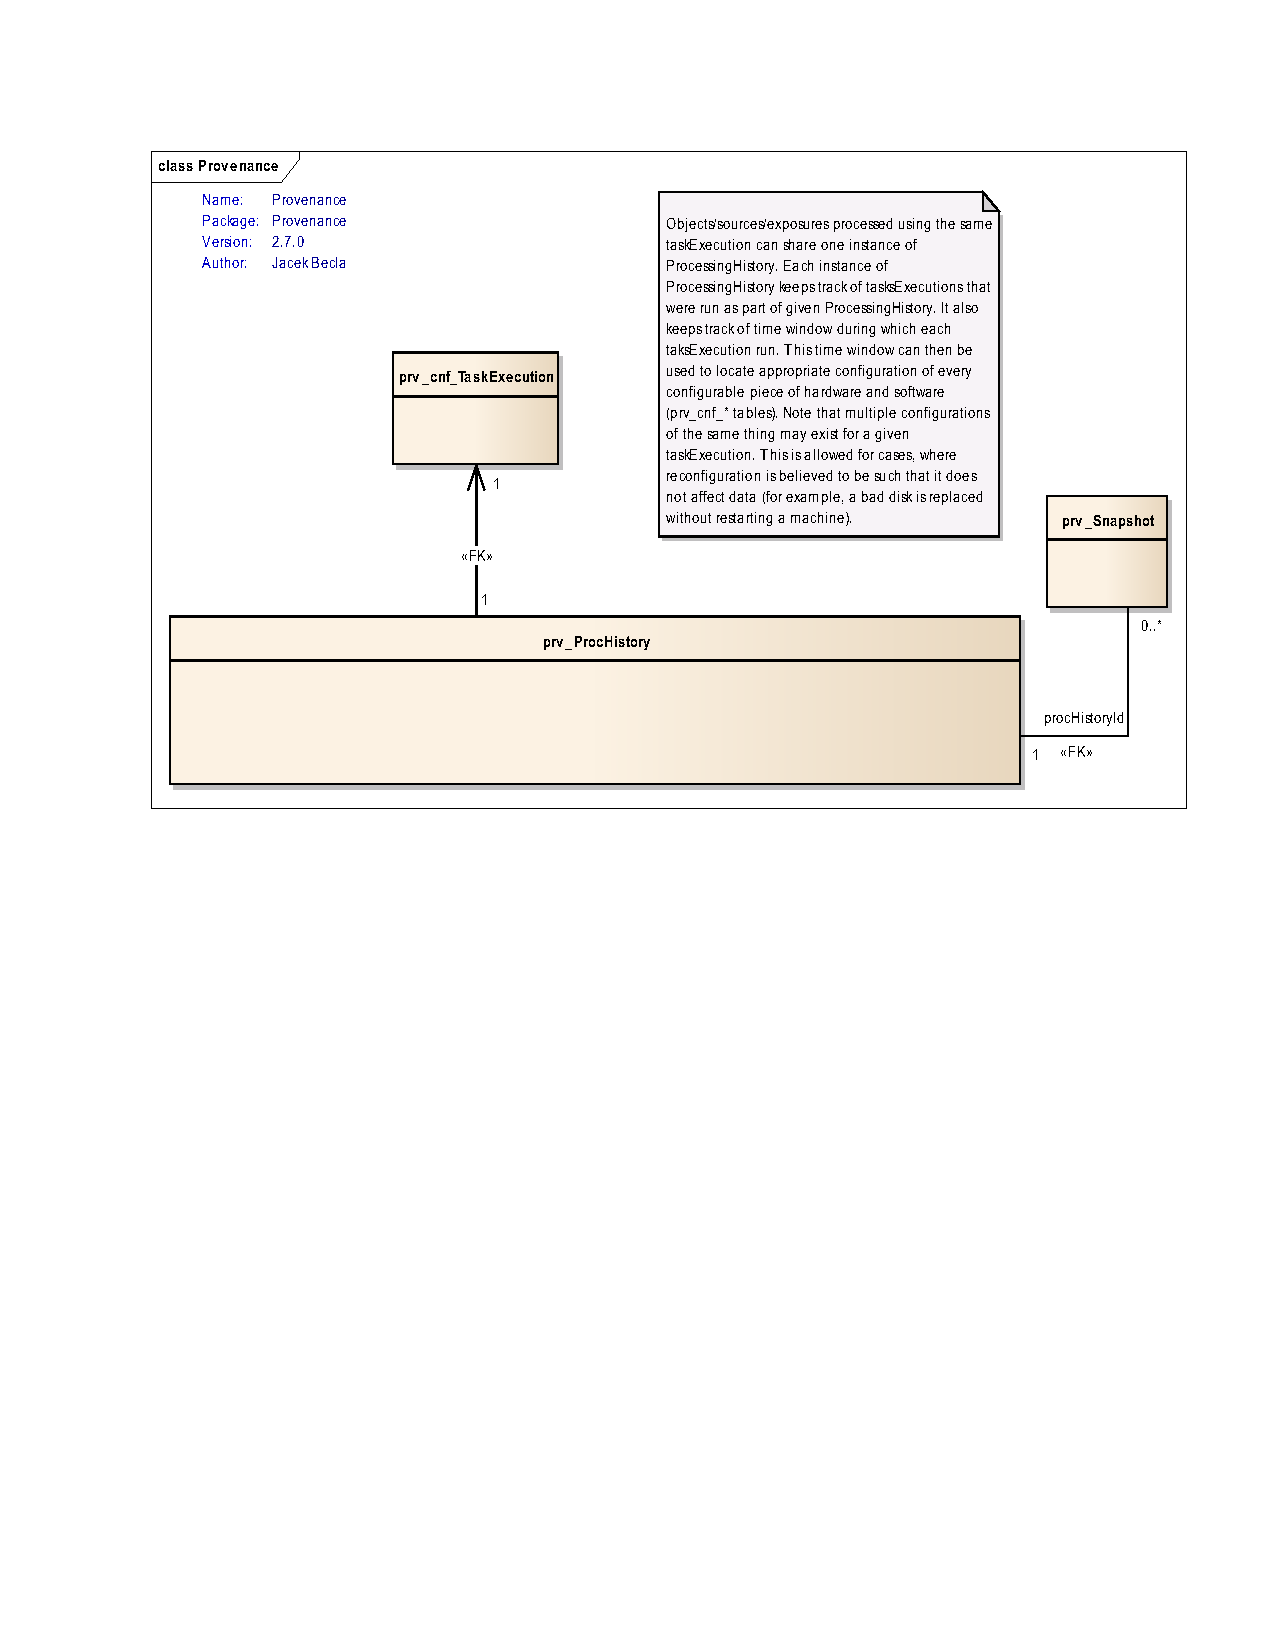
\includegraphics[scale=0.80]{diagrams/provenance}
  \caption{Provenance table relationships}
\end{figure}

\begin{figure}
  \centering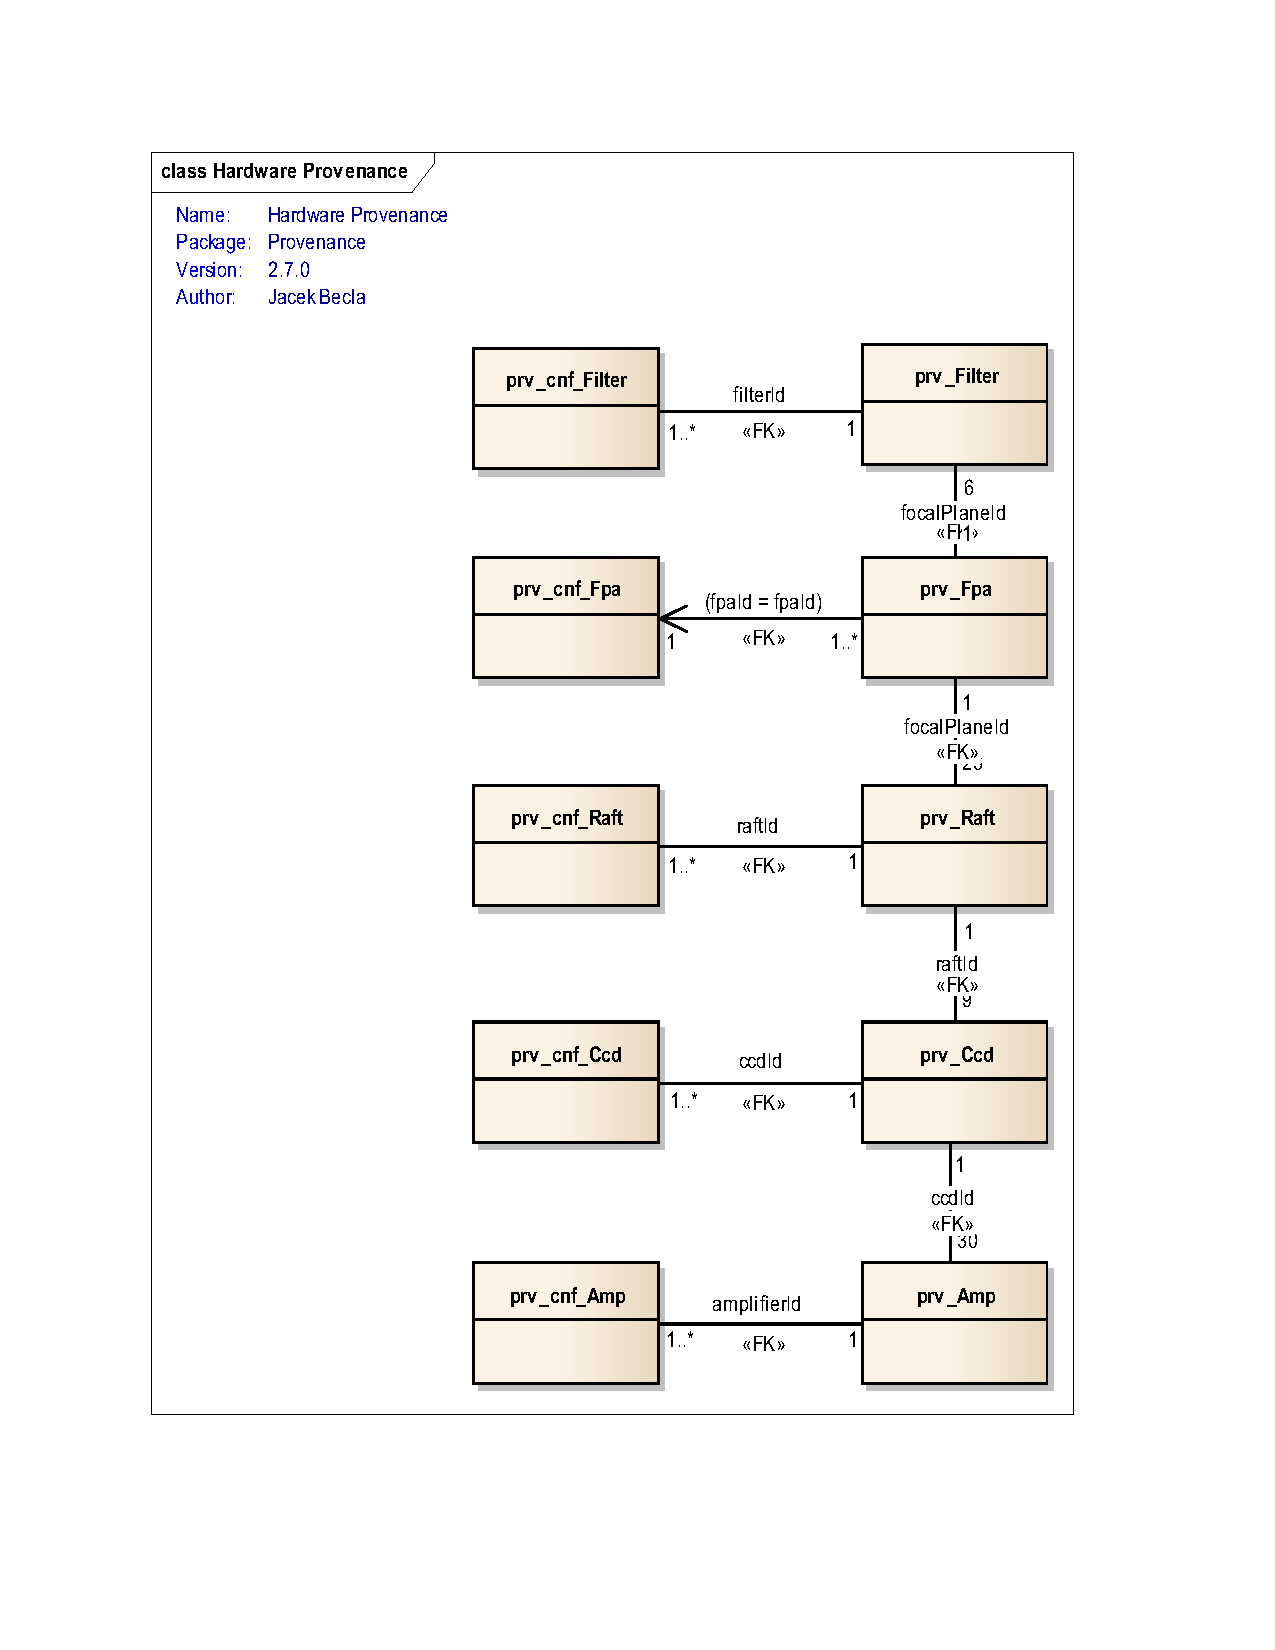
\includegraphics[scale=0.70]{diagrams/hardware_provenance}
  \caption{Hardware provenance table relationships}
\end{figure}

\begin{figure}
  \centering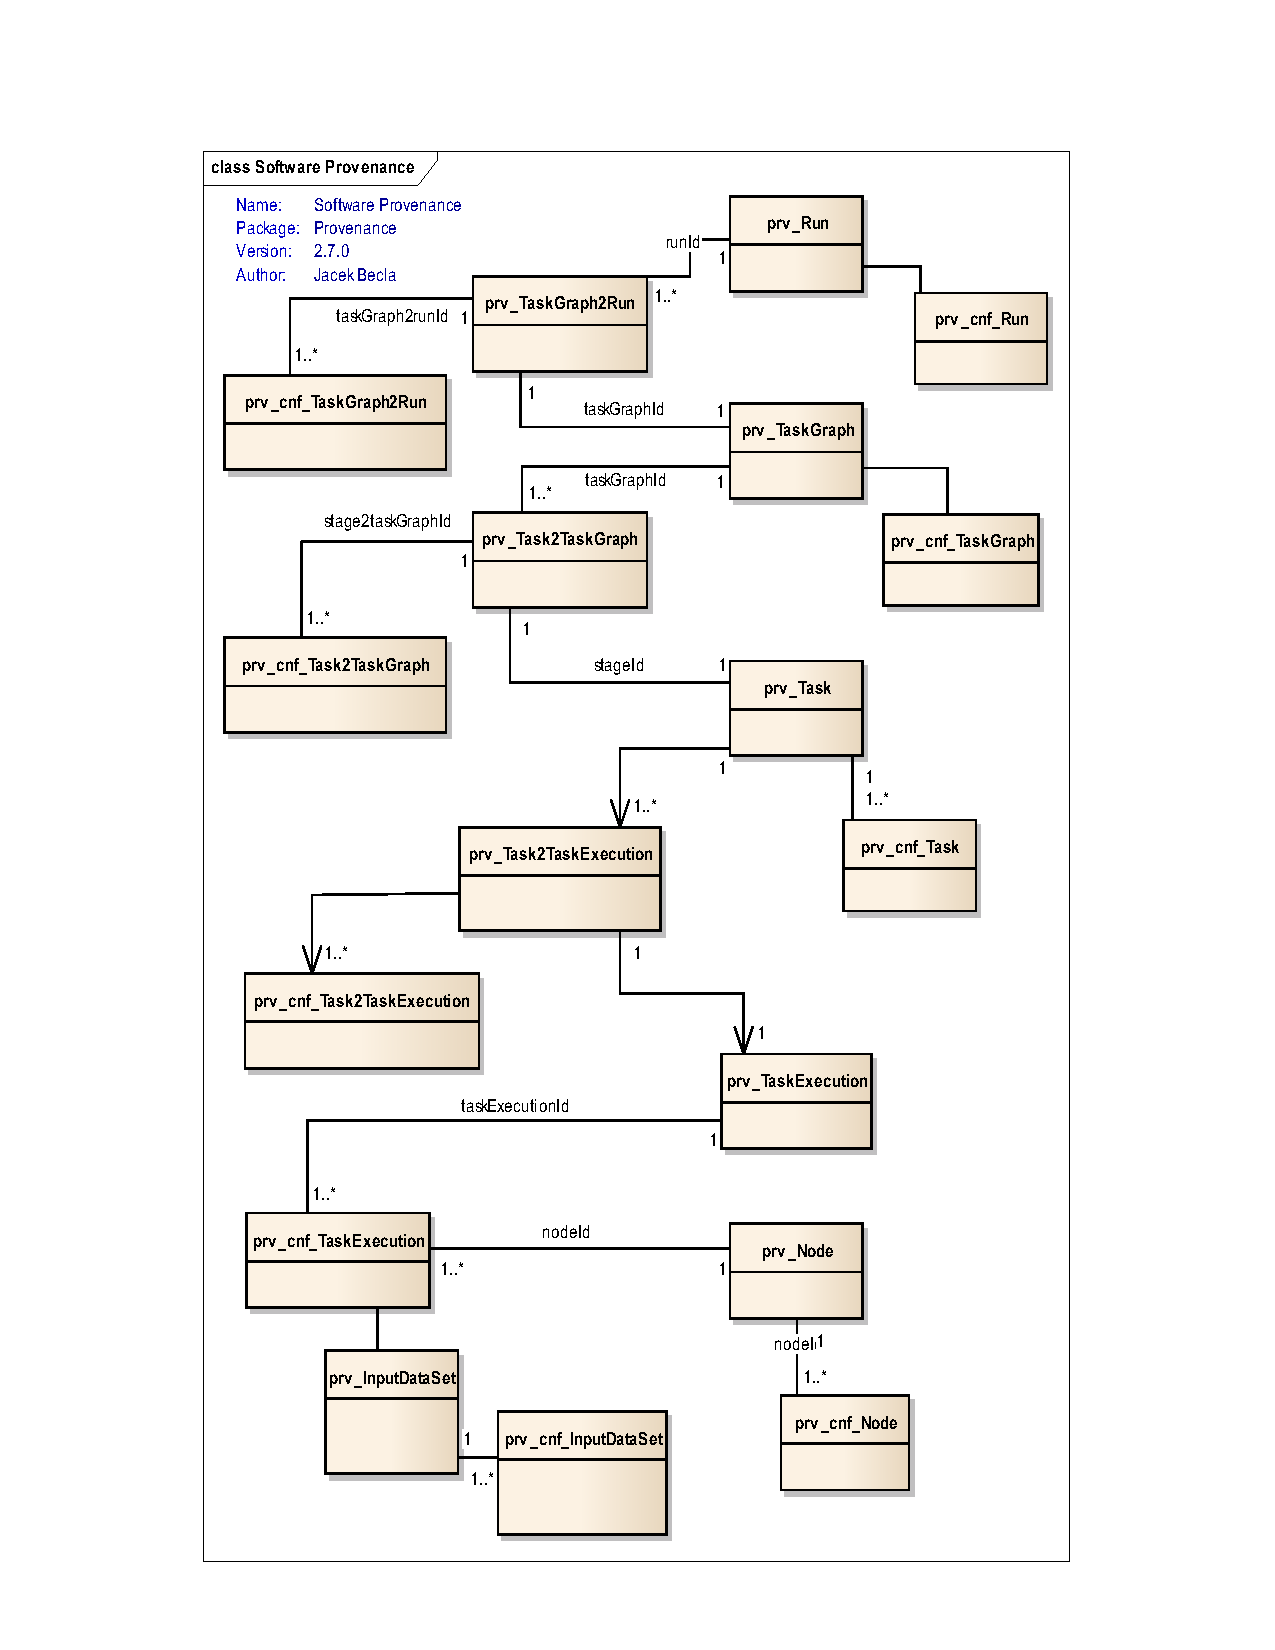
\includegraphics[scale=0.70]{diagrams/software_provenance}
  \caption{Software provenance table relationships}
\end{figure}

\subsection{Other Tables}

In addition to the catalogs/tables described above, there are several groups of other tables in the baseline schema. In terms of size and complexity they pose very little challenge comparing to the catalogs described above, thus this document does not focus on discussing these tables (and we have left designing details of these tables for closer-to-commissioning). They include Software Data quality Assurance tables (prefixed with sdqa\_), used for tracking various quality aspects of the LSST catalogs.

\section{Selected Design Aspects}

Below we covered in details selected, most interesting aspects of the schema design.

\subsection{Provenance}

Provenance is fundamentally concerned with two things: recording the state of relevant portions of the system and associating state with the generation of an output from inputs. Given the size of data, provenance information cannot be captured per data element. Instead data elements with the same provenance should be grouped. That in turn is non-trivial due to the way data elements will be built and updated:

\begin{itemize}
  \item Any given data element will be the result of the processing of raw data by a Task Graph (also called a pipeline). Each Graph consists of many Tasks. Each task may involve executing multiple algorithms.
  \item It is anticipated we will need to fix bad data (as long as it is unreleased) by reprocessing it (e.g. using a fixed algorithm), so in practice different parts of the same data element might have many different processing histories.
  \item Finally, there is a large number of dependencies. Here is just a small example: object data depends on a coadd, which is generated using masks derived from difference sources which depend on the corresponding difference image which depends on a template image which depends on calibrated science images and so on...
\end{itemize}

Also, provenance should be flexible enough to easily allow adding new items to the system state.

For the above reasons, simple solutions like timestamping every data element will not work.

In practice, we plan to implement the state recording function of Provenance using time ranges, with granularity up to 1 sec. Every configurable piece of information will be tracked through two tables: one that keeps definitions and the other that keeps configurations. For example, each filter (u, g, r, i, z, y) will be represented as one row in prv\_Filter table (there will be exactly 6 definitions), and each configuration of each filter will be represented as one row in prv\_cnf\_Filter table (initially there will be 6 configurations: one for each filter, but if we happen to later break one filter and will introduce a new one, a new configuration will need to be inserted). Each configuration will have a validity time range assigned (time period when it was valid).

The heart of the processing recording function of Provenance is the \textit{prv\_ProcHistory} table; it has two responsibilities:

\begin{itemize}
  \item Assign a unique processing history id (procHistoryId) for each creation of a set of output data elements. An 8-byte integer is sufficient to provide the needed granularity.
  \item Bind each unique procHistoryId with a set of executions of tasks, including the inputs to those tasks, identified by their own procHistoryIds. (A task is the smallest chunk that will be executed atomically, that is, if part of a task fails, the whole task will be rolled back and re-run). Typically there will be one task execution for each procHistoryId, but in cases of reprocessing there may be more than one.
\end{itemize}

Notice that procHistoryId is not associated with a time range, but with a set of task executions, each having its own configuration, its own time range, and its own node it runs on.

The Provenance may also track which columns for each table are updated by each stage (we require that each column is updated by a single stage only - for that reasons some columns, eg. flags had to be split into multiple columns).

Every data element that needs to have provenance tracked (for example, every row in the Object, Source, or Exposure table) will need to store a procHistoryId. Note that a single row might be generated or updated by different pipelines or task graphs, and each may run at different time, on different hardware, possibly even at a different site. Having a procHistoryId will allow it to find which task graphs and tasks were executed for it, at what time, and on which processing nodes. It will then be possible to correlate the time periods when each task was executed with the configurations that were valid at those times.

Such an approach has two important pros:

\begin{itemize}
  \item \textbf{Flexibility}: It allows us to decouple configurable elements from Objects, Sources, Exposures, etc. --- they are very loosely coupled through time range only. In particular, it means that new configurable items can be added or removed from the system at any given time with no need to do schema evolution and no need to update existing data.

  \item \textbf{Space-efficiency}: It is clear that components of the system will be changing relatively frequently. Minimizing the storage required to track these changes is essential. In our case, a new configuration will only require storage for that configuration. Each Object/Source/Exposure only needs to store one procHistoryId to get access to hundreds of different configurations.
\end{itemize}

We expect we will need to tune the current approach to provide efficient query access to the Provenance. In particular, the implementation relies on range queries which may need special optimizations, or special indexes.

\subsection{Schema Evolution}

In summary, we expect to avoid heavy changes that alter shape of large tables (e.g. by preallocating space), and rely on partitioning to scale and run necessary schema changes fast and scalably in parallel\footnote{For more information about the schema evolution tests we run, refer to https://dev.lsstcorp.org/trac/wiki/db/tests/SchemaEvolution}.

\subsubsection{Released Data Sets}

Each data release is independent, therefore the database schema can easily change between data releases; we do not anticipate any non-trivial challenges here.

\textbf{Adding new columns}. We are planning to keep a few extra unused columns of each common type (for example, 3 FLOATs, 3 DOUBLEs, 3 INTs, 3 BIGINTs) for each large table, and use one of them when a new column is needed. (renaming a column is a trivial and instantaneous operation). Speed of filling new columns should be comparable to speed of a full table scan.

\textbf{Updating existing columns}. Speed of updating values should be comparable to speed of a single shared scan.

\textbf{Deleting columns}. If we have to delete a column, instead of deleting it, (which is expensive as it changes shape of a table), we will add it to the pool of "extra, unused columns" by renaming it.

The unsed/hidden columns will be hidden through non-materialized views. It is likely that we will end up providing multiple views, e.g. each time we make a schema change, we'd expose the changes through a new view.

\textbf{Non-trivial changes}. Should we ever need to do non-trivial changes: Non trivial schema changes on multi-billion row table tend to take extremely long time (measured in days). In our case, each large table will be partitioned into several thousand chunks, which makes the updates scalable and faster: not only the updates can be done in parallel on multiple machines, but each partition is small enough to be handled efficiently without running into any bottlenecks or problems with lack of buffer space.

\textbf{Notes on administration}. All queries accessing the database will go through our interface, which intercepts and interprets the queries. This will allow us to put the entire system in special mode (user queries will be queued, administrative queries will continue to work). The administrative tools we are building will allow us to push the necessary updates to all nodes, and we could use the existing scheduling mechanisms to run the upgrade in the most efficient fashion. The admin tools will also allow running necessary verifications (e.g., whether the schema for all table chunks matches).

\subsubsection{Level 1 (Up-to-date Catalog)}

We will have opportunity to update schema every time we are replacing Level 1 catalog after each data release. Should we need to make the updates in between, the changes can easily be done during the time when we are not taking data (daytime).

\section{Naming Conventions}

We have defined a set of naming convention for naming tables, columns and relationships. In summary, the format of table names follows: 

\texttt{<\_><prefix><purpose>\_<extend>\_<component><postfix>}

Leading \_ is used to show it is an internal table.

Prefix:
\begin{itemize}
  \item All Provenance tables are prefixed with prv\_, example: prv\_Amp. Further, it may be followed by cnf\_ which is used for provenance tables containing individual configurations. For example, one row in prv\_Ccd contains information about one particular Ccd, and prv\_cnf\_Ccd contains information about one specific configuration version of one particular Ccd.
\end{itemize}

Purpose: it includes things like Raw, Science, Calibration, Bias, Dark, Flat, Fringe, IR. (we have recently dropped ``Science'' for *Visit tables).

Extend: Fpa, Ccd, Amp (we have dropped ``Fpa'' from raw and science table names).

Component: Exposure, Object, Source, Psf, Wcs...

Postfix: optional

Mapping tables follows its own naming scheme: \_<table X name>\_To\_<table Y name>


\section{Baseline Schema}

\input{version_string}

\rowcolors{2}{gray!25}{white}
\input{core_tables}

\rowcolors{2}{white}{white}
\appendix
% Include all the relevant bib files.
% https://lsst-texmf.lsst.io/lsstdoc.html#bibliographies
\section{References} \label{sec:bib}
\bibliography{lsst,lsst-dm,refs_ads,refs,books}

%Make sure lsst-texmf/bin/generateAcronyms.py is in your path
%\section{Acronyms used in this document}\label{sec:acronyms}
%\input{acronyms.tex}
\end{document}
